\section{Middleware}

\subsection{Was ist Middleware}

Eine Middleware ist eine Technologie, die die Kommunikation über ein Netzwerk ermöglicht und auf Sockets basiert. Von einer Middleware werden gewisse Funktionalitäten erwartet, die sie von der bloßen Netzwerkkommunikation unterscheiden:

\begin{itemize}
    \item Es wird eine Infrastruktur mit Lösungen für Standardaufgaben bereitgestellt.
    \item Es wird Verteilungstransparenz z.B. Ortstransparenz ermöglicht.
    \item Es werden ggf. zusätzliche vom Einsatzbereich abhängige Funktionalitäten bereitgestellt.
\end{itemize}


\subsection{Message-oriented Middleware}

Die Message-oriented Middleware (MoM) überträgt - so wie der Name es schon verrät - Daten als einzelne Nachrichten. MoMs bieten die folgenden Features:

\begin{itemize}
    \item Warteschlangen (queues) für die Zwischenspeicherung von Nachrichten
    \item Infrastruktur zur Benennung von Kommunikationsendpunkten, also einen Namensdienst, der Kommunikationspartner anhand von Namen oder IDs anstatt von IP-Adresse und Port identifiziert.
    \item Funktionen zur Akkumulierung von Nachrichten. Einzelne Nachrichten können automatisch akkumuliert werden und nur das Ergebnis übertragen werden.
    \item Direkte Unterstützung von Broadcast ohne spezielle IP-Adressen
\end{itemize}

Der Nachrichtentransfer über MoM ist asynchron und wird auch \textbf{Message Passing} genannt. Die Daten werden beim Senden in eine Warteschlange gegeben und bei Bedarf abgefragt. Auf diese Weise können Nachrichten zu jeder Zeit gesendet und empfangen werden ohne darauf zu warten, dass der Kommunikationspartner bereit ist.\\
Auf diese asynchrone Kommunikation kann man bei Bedarf natürlich eine synchrone Kommunikaiton aufbauen, indem man z.B. ein Request-Reply-Modell implementiert.

Im folgenden wollen wir nun Beispiele für MoM kennenlernen, um besser zu verstehen, wie eine MoM aussehen kann.

\subsubsection{MQTT}

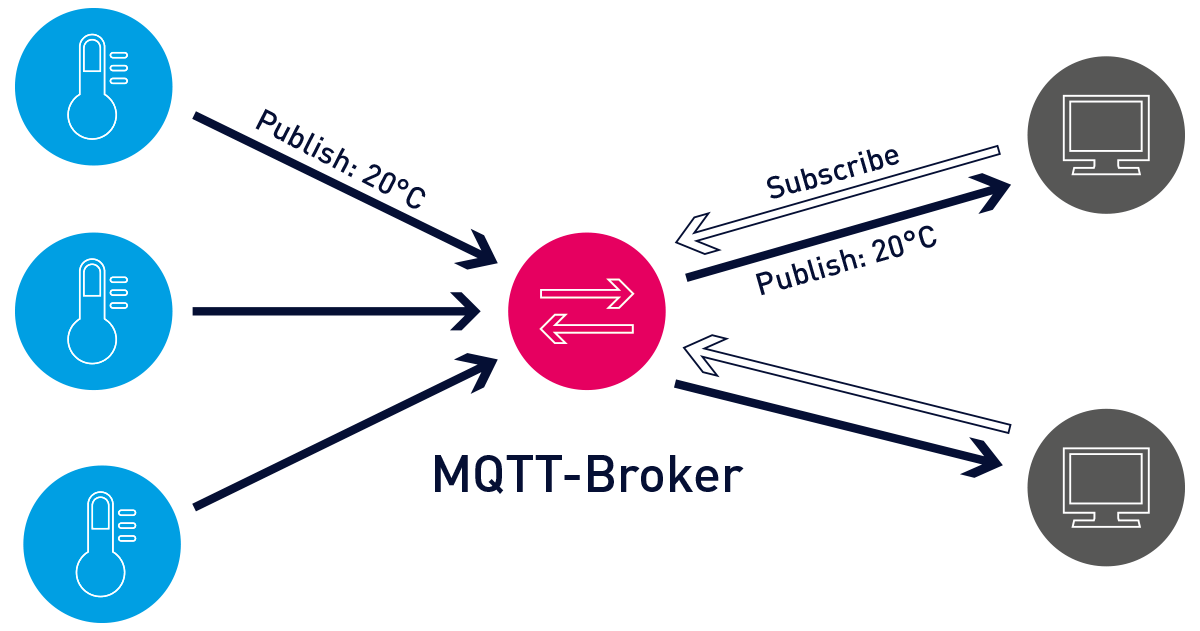
\includegraphics[height=170px]{MQTT.png}

Bei MQTT gibt es einen Broker, der der Nachrichten empfängt und ausliefert. Er enthält eine Warteschlange und optional eine Datenbank in der Nachrichten persistent gespeichert werden können. Die Publisher müssen sich beim MQTT-Broker registrieren und können dann Nachrichten an ihn senden. Die Subscriber können dann diese Nachrichten abfragen. Nachrichten können einem gewissen \textit{Topic} zugeordnet werden. Topics sind eine Einteilung in semantische Gruppen von Nachrichten. So können Subscriber dann nur Nachrichten zu den Topics abfragen, die für sie interessant sind.\\
Die Publisher und Subscriber müssen nur noch die IP-Adresse des Brokers kennen. Der Broker implementiert Logik, um sich zum Zeitpunkt der Registrierung die IP-Adresse des Teilnehmers zu merken. Somit entsteht Ortstransparenz. Nur der Broker kennt nun die genauen Teilnehmer. Die anderen Komponenten des verteilten Systems senden und empfangen jetzt Nachrichten ohne zu Wissen zu wem sie gelangen oder von wem sie kommen. Man kann nun für den Broker eine vorgegebene Implementierung, wie Mosquitto, benutzen. Auf diese Weise muss man sich mit dem Teil, der die Logik der Middleware implementiert, nicht mehr kümmern und kann die vollen Vorteile der MoM ausspielen.\\
MQTT wird vor allem gerne im Zusammenhang mit dem IoT und Sensoren genutzt.

\subsubsection{MPI \& MPICH}

MPI (Message Passing Interface) ist ein Standard, der den Nachrichtenaustausch bei parallelen Berechnungen in verteilten Systemen betrifft. MPI ist folglich im Zusammenhang mit High Performance Computing (HPC) relevant, also dort, wo enorme Rechenlast auf Cluster verteilt werden soll. Dabei sind alle Rechenprozesse meist gleichartig, führen also den selben Code mit unterschiedlichen (Teil-)Daten aus. MPICH ist eine Implementierung dieses Standards.\\
MPICH stellt ein CLI zur Verfügung mit dem mehrere Instanzen eines Programms zur Parallelen Ausführung gestartet werden können. Z.B.:\\
\textbf{\$ mpiexec -n 36 ./myProgram}\\
In dem Programm selbst kann man dann die MPICH Bibliothek benutzen, um die Kommunikation zwischen den Prozessen zu implementieren. Das CLI übergibt den Prozessen als Parameter dann weitere Informationen, die im Programmcode dann durch einen einfachen Aufruf von MPI\_Init genutzt werden, um das MPI des Prozesses zu initialisieren. Dazu gehört auch eine ID. Man kann dann sein Programm so schreiben, dass alle Prozesse eine Berechnung durchführen und ihr Ergebnis an den Prozess mit ID=0 schicken, der dann alle Ergebnisse ausgibt. Für die einfache Akkumulierung von Werten, z.B. Summen- oder Produktbildung, kann direkt beim Senden der Daten ein Funktionsaufruf benutzt werden, der die Akkumulierung durchführt und nur das Ergebnis an den Empfänger überträgt. MPI hat den Anspruch fehlerfreier Nachrichtenübertragung. Falls ein interner Fehler auftritt, wird die Übertragung erneut versucht bis sie erfolgreich ist (retransmission). Das bedeutet, dass der Programmierer sich nicht um Fehlerbehandlung kümmern muss (Fehlertoleranz), aber auch, dass er auch keine Fehlerbehandlung durchführen könnte, wenn es doch zu internen Fehlern kommt (Kontrollverlust). Es folgt ein kurzes Programmierbeispiel:

\begin{lstinputlisting}[language=C++]
    {../src/MPICH/main.cpp}
\end{lstinputlisting}

\subsubsection{Apache Kafka}

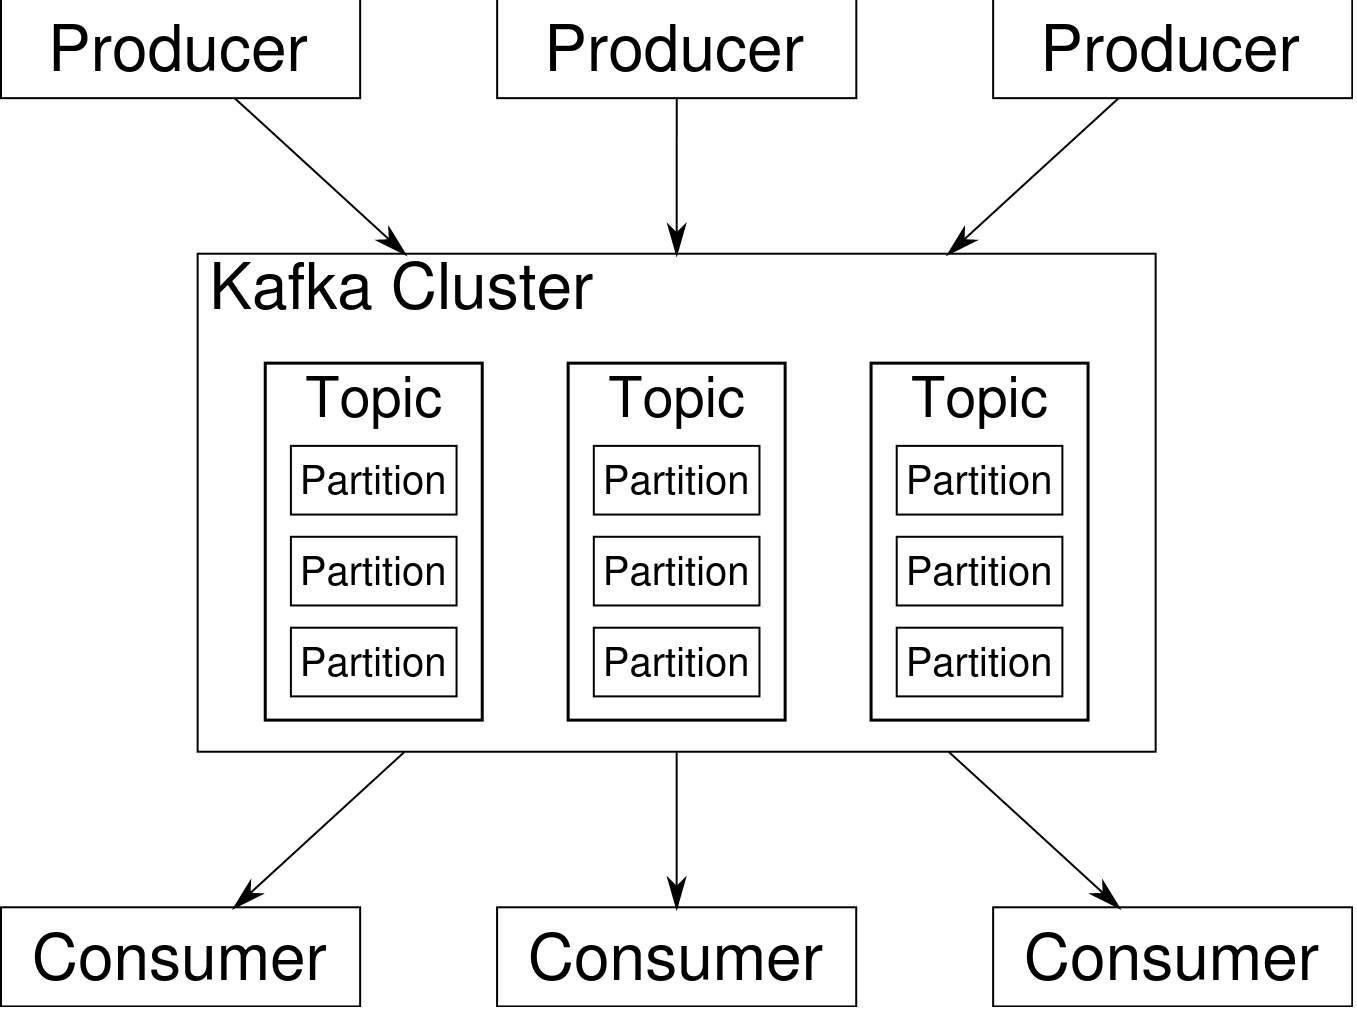
\includegraphics[height=170px]{ApacheKafka.png}

Apache Kafka ist eine Open Source Middleware, die ähnlich wie bei MQTT ein Publish-Subscribe System implementiert. Der wesentliche Unterschied ist, dass Kafka statt Nachrichten Datenströme verarbeitet und auf High-Performance und High-Scalability ausgelegt ist. Ursprünglich von der Firma LinkedIn entwickelt sollte Kafka dazu verwendet werden, Logging Daten von sehr großen Rechnernetzen in Echtzeit zu sammeln. Mit den gesammelten Daten konnten dann Echtzeit-Analysen über das Gesamtsystem erstellt werden.\\
Bei Kafka gibt es, wie bei MQTT, Publisher/Producer, Subscriber/Consumer und Broker. Bei Kafka können die Broker und die Subscriber geclustert werden, um Ausfallsicherheit und hohe Skalierbarkeit zu gewährleisten.

\subsection{Object-oriented Middleware}

Object-oriented Middleware ist eine Gruppe von Middleware, bei der Objekte einer Programmiersprache übertragen werden können. Im folgenden wollen wir die Java RMI (Remote Method Invocation) betrachten.\\

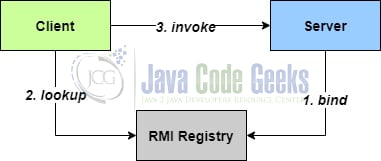
\includegraphics[height=100px]{JavaRMI.jpg}

Es gibt einen Server, der Objekte mittels bind/rebind unter einem gewissen Namen bei der RMI Registry veröffentlichen kann. Die Objekte, die der Server bei der RMI Registry veröffentlicht, müssen ein Interface implementieren, das vom Interface Remote erbt. Clients können über eine Methode lookup veröffentliche Objekte bei ihrem Namen in der RMI Registry finden und so Referenzen auf sie erhalten. Der Client kann dann die Methoden des Remote Interfaces auf dem Objekt aufrufen, wodurch der Code auf dem Rechner ausgeführt wird, der das Objekt veröffentlicht hat. Hier ist es ganz normal möglich Objekte als Parameter oder Rückgabewert zu benutzen. RMI überträgt also die Objekte mit dem Bytecode.\\
Mit RMI können z.B. auf einfache Weise Rechenservices implementiert werden, indem der Server ein Objekt mit einer Methode bereitstellt, die ein beliebiges Objekt übernimmt, einen in dem übergeben Objekt definierten Taks ausführt, und den Rückgabewert zurückgibt. Der Client kann dann die Methode des Server-Objektes mit seinen eigenen Objekten, also Tasks, als Argumente aufrufen.\\

\textbf{Fazit:} Bei OoM wird von Client und Server initial die IP-Adresse des Brokers benötigt. Sonst brauchen Server und Client aber keine Kenntnis darüber haben, wo sich ihre Kommunikationspartner befinden und wie viele es gibt. Daher ist OoM verteilungstransparent. Der Zugriff auf Ressourcen wird durch OoM ebenfalls sehr einfach.

\subsection{Web Services}
\subsubsection{SOAP, UDDI, WSDL}

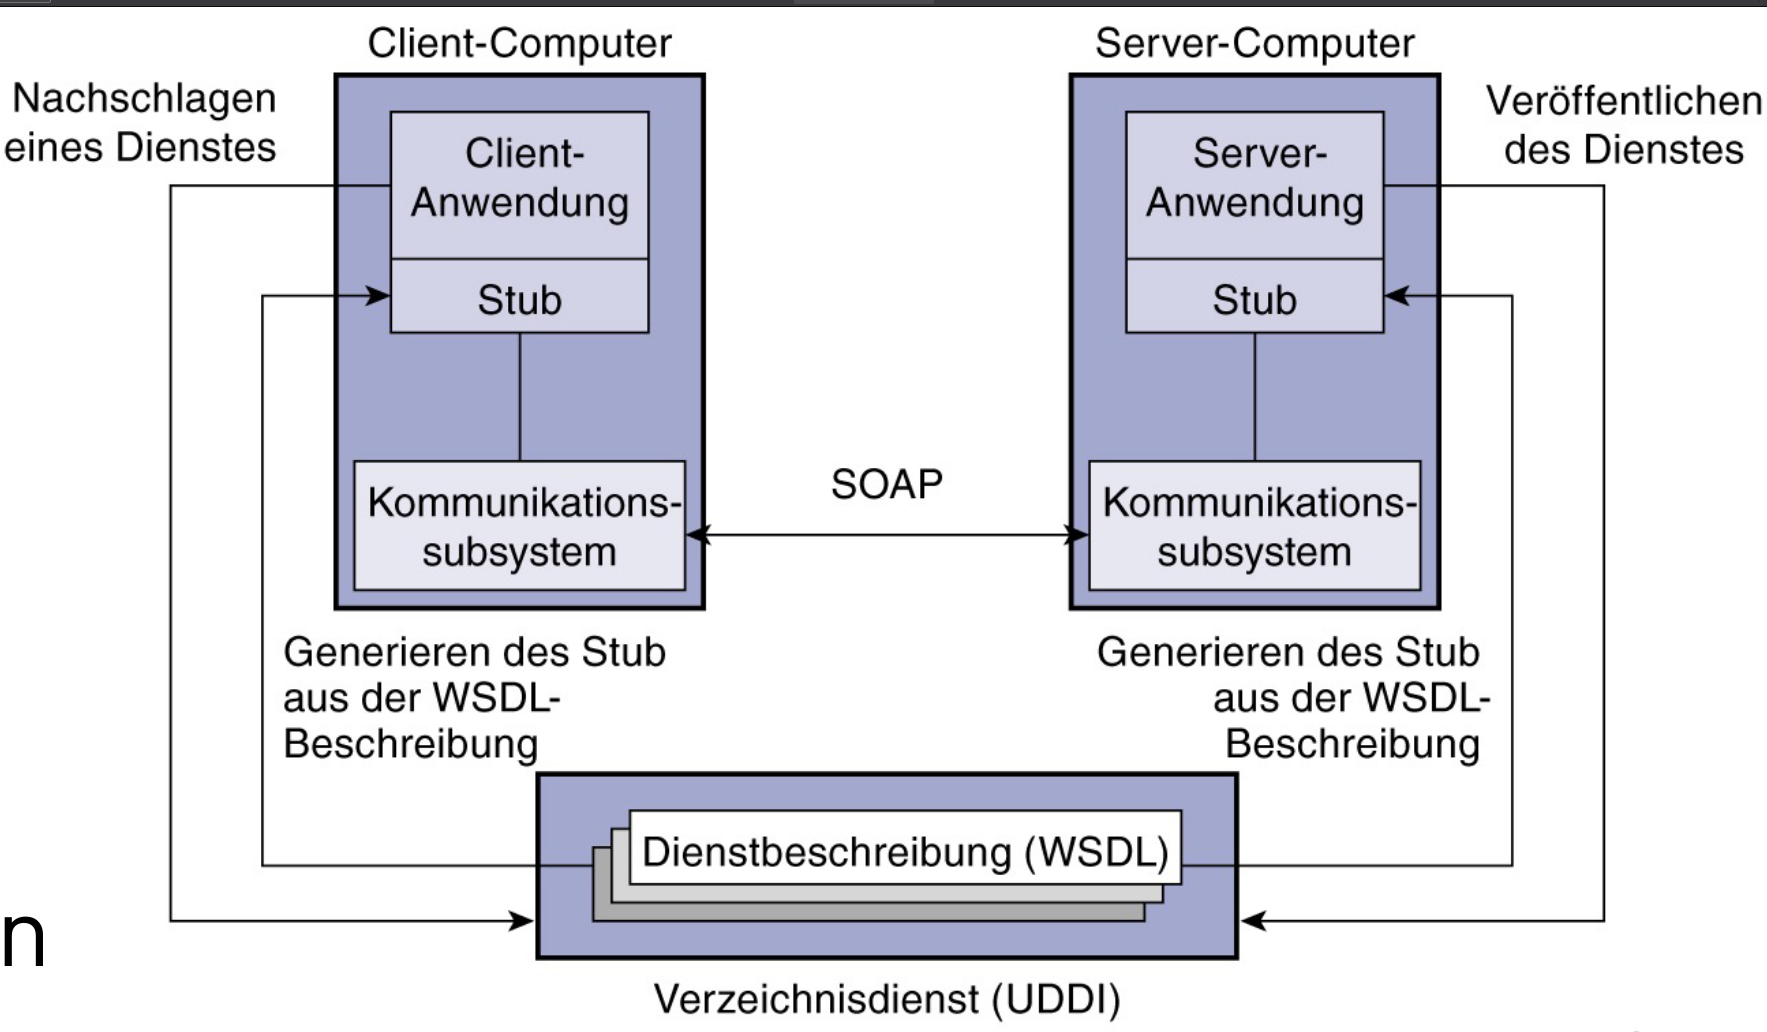
\includegraphics[height=200px]{SOAP.png}

SOAP steht für Simple Object Access Protocol und ist ein XML basiertes Protokoll zur Bereitstellung von Webservices, das gewöhnlich HTTP als Trägerprotokoll nutzt.\\
Die wesentlichen Dinge, die in einer Infrastruktur, die SOAP nutzt, wichtig sind, sind  WSDL (Web Service Definition Language) und UDDI (Universal Description, Discovery and Integration).\\
Die Beschreibungssprache WSDL wird genutzt, um zu definieren welche Funktionalitäten ein Webservice bereitstellt. Diese Schnittstellenbeschreibung wird auf einem Verzeichnisdienst, der UDDI-Registry, hinterlegt. Aus der WSDL können direkt sog. Stubs generiert werden. Das sind generierte Funktionen oder Klassen in einer bestimmten Programmiersprache, z.B. Java, die von Anwendungen benutzt werden können und SOAP implementieren. SOAP selbst ist ein XML-basiertes Protokoll in dem Anfragen und Antworten an/von den Services kodiert werden können. Das ist also ähnlich wie bei RPC-Frameworks, wo auch aus einer gemeinsamen Schnittstellenbeschreibung Code für Server und Client generiert wird.\\
Die Veröffentlichung einer WSDL Beschreibung und das auffinden dieser verläuft über die die UDDI-Registry. Die Kommunikation selbst verläuft dann aber ohne Umweg zwischen Client und Server.

\textbf{Fazit:}
UDDI bringt eine gewisse Ortstransparenz, da Client und Server nur die Schnittstelle über die UDDI-Registry erfahren müssen und dann ohne wissen über den Standort miteinander kommunizieren können.

\subsubsection{REST}

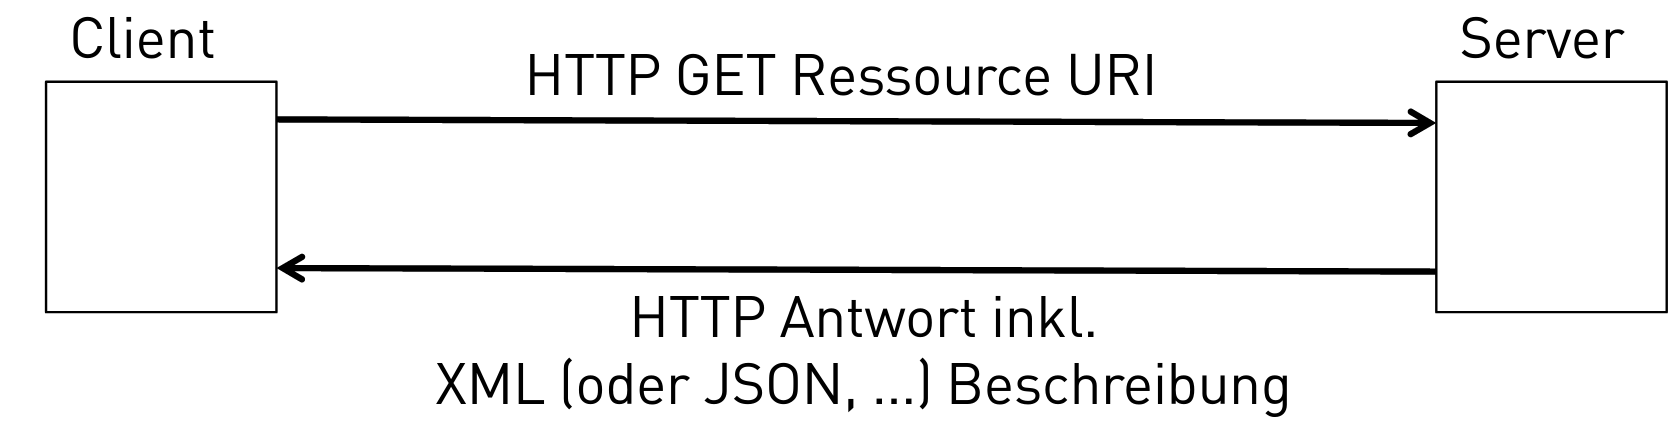
\includegraphics[height=80px]{REST.png}

REST (REpresentational State Transfer) kommt ursprünglich aus einer Doktorarbeit von Roy Fielding im Jahr 2000. Dort hat er beschrieben, wie alle CRUD Operationen eines Web-Services mittels HTTP GET, POST, PUT, PATCH, DELETE durchgeführt werden sollen können. Die Parameter und die Rückgabewerte werden in einem standardisierten XML-Format kodiert.\\
Heutezutage haben wir meist ein etwas anderes Verständnis von REST. REST ist inzwischen meist einfach eine Bezeichnung dafür, dass ein HTTP GET an eine bestimmte URL geschickt wird, die bestimmt was der Aufruf bewirken soll. Der Name des Services und die Parameter werden also in der URL kodiert. Falls es eine Antwort mit Daten gibt, wird sie oft in JSON kodiert.\\
Ein gutes Beispiel für eine URL, die auf eine REST API verweist ist:\\
https://api.twitter.com/1.1/statuses/mentions\_timeline.json?count=2\&since\_id=14927799\\
Hier werden z.B. recht offensichtlich die ersten 2 Stati seit der id=14927799 von der API verlangt.\\

\textbf{Fazit:}
REST ist sehr leichtgewichtig und einfach zu verstehen und umzusetzen. Es bietet einfachen Zugriff auf Ressourcen, sorgt jedoch nicht viel für Transparenz. Der Client muss dennoch den genauen Namen des Servers und die URLs seiner bereitgestellten Services kennen. Ein Fortschritt in der Transparenz ist jedoch, dass der Client nur noch den Hostnamen des Servers kennen muss und sich nicht mehr um Ports kümmern muss, da der Port 80 implizit angenommen wird. Da REST mit einfachen Mitteln gebaut ist liefert es auch Offenheit.